\section{Aufbau der Stoffe} {SW 1-2}

\subsection{Inhalt}
\begin{itemize}
\item Atomaufbau
\item stoffmodelle
\item reinstoffe und gemische
\item isotope
\end{itemize}
            
\subsection{Stoffe}	

\renewcommand{\arraystretch}{1.2}
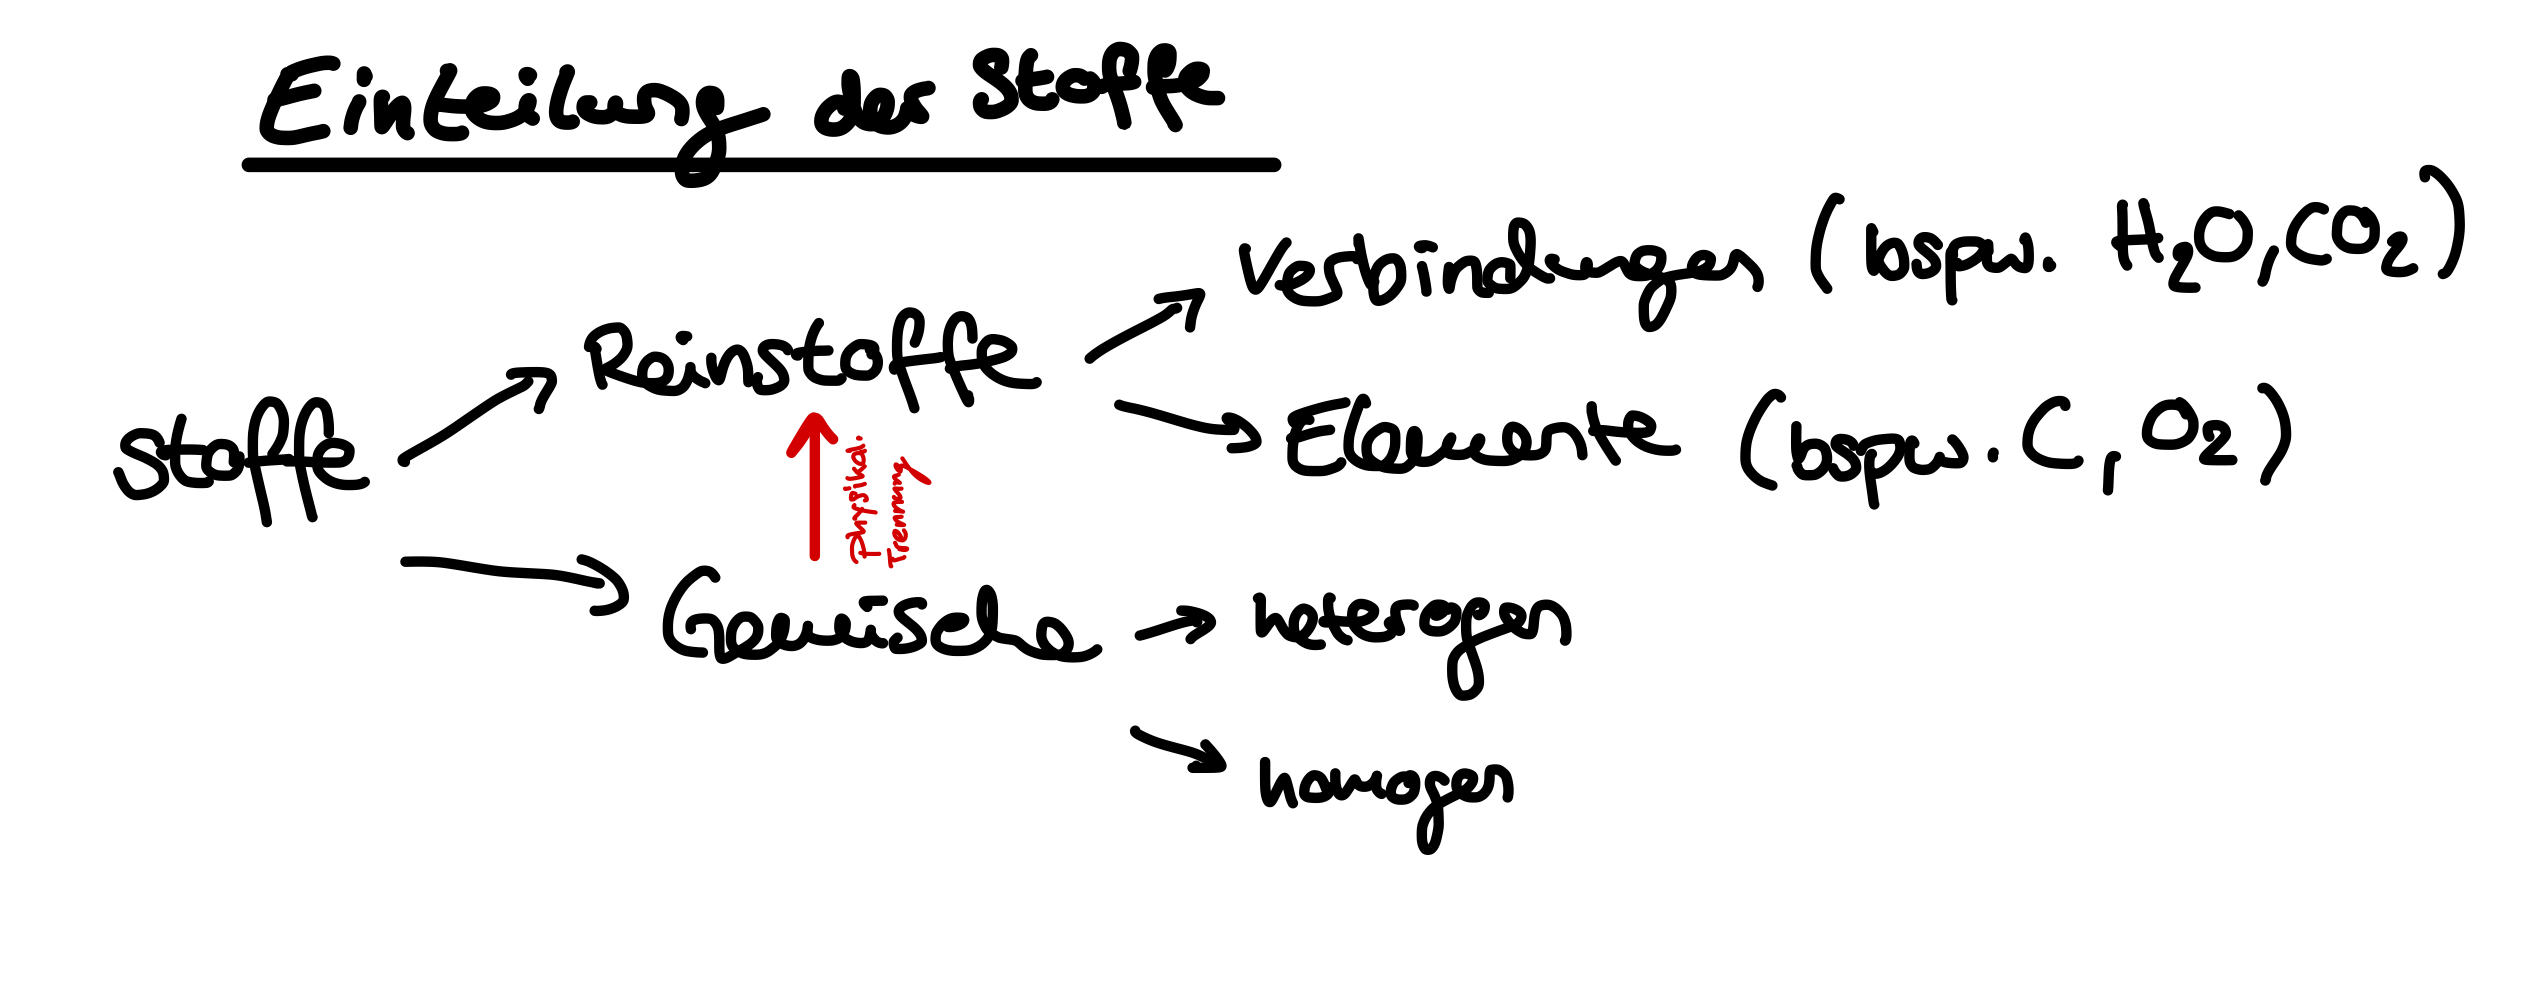
\includegraphics[width=9cm, height=3cm]{images/Stoffe.png}

\subsection{Aggregatzustand}		

{\tiny
\begin{tabular} {ll | ll} 
	Aggregatzustand  	&     					& Dispersitätsgrad    &  \\ 
	Dispersionsmittel  	& Dispergierter Stoff	& Heterogen   		& Homogen        \\
	gasförmig (g) 		& gasförmig (g)        	& -          		& Gasgemisch        \\
	gasförmig (g)		& flüssig (l)			& Nebel				& -		\\
	gasförmig (g)		& fest (s)				& Rauch				& -		\\
	flüssig (l)			& gasförmig (g) 		& wenig haltbarer Schaum	& Gaslösung		\\
	flüssig (l)			& flüssig (l) 			& wenig haltbare Emulsion				& Glüssigkeitslösung		\\
	flüssig (l)			& fest (s) 				& Suspension				& feststofflösung	\\
	fest (s)			& gasförmig (g) 		& fester Schaum ( zB. Schaumstoff)					&		\\
	fest (s)			& flüssig (l) 			& brei				&		\\
	fest (s)			& fest (s) 				& Feststoffgemische				& legierung zweier Metalle	\\
	
\end{tabular}
}

\subsection{Eselsbrücke}

\begin{tabular}{ll} 
    HONClBrIF – "der Brief vom Onkel"   &  Die Buchstaben stellen dabei \\
     & die Elemente des Periodensystems dar,\\
     & die in der Natur nur 2-atomig vorkommen. \\
    Ausnahme: & $P_4$ (Phosphor) und $S_8$ (Schwefel)  \\
\end{tabular}
\renewcommand{\arraystretch}{1}      
         

\subsection{Kugelwolkenmodell}	

\subsection{Isotope}

  
           